% Section content template for individual Educative lessons
% This file contains the actual content for a specific section
% Generated from Educative API section content

% Section: Class Diagram for the Chess Game
% Section ID: 5732015845670912
% Section Slug: class-diagram-for-the-chess-game
% Generated: 2025-12-12T16:11:17.429647

In this lesson, we'll create the class diagram for the online chess game. We 'll follow a bottom-up approach: design the simplest components and build up to the core game classes, showing relationships and responsibilities throughout.

\subsection{Components of chess}\label{bAQ1eGrRCcgjmA0xhjU84}
\\
As mentioned earlier, we'll follow the bottom-up approach to designing a class diagram for the chess game.

\subsubsection{Box}\label{7Z2W6AocpLQ4PlcGHlmvV}
\\
A \texttt{Box} represents a position on the 8x8 chessboard, defined by a row and column (0--7). It may either be empty or occupied by a chess piece.

\begin{figure}[htbp]
 \centering
 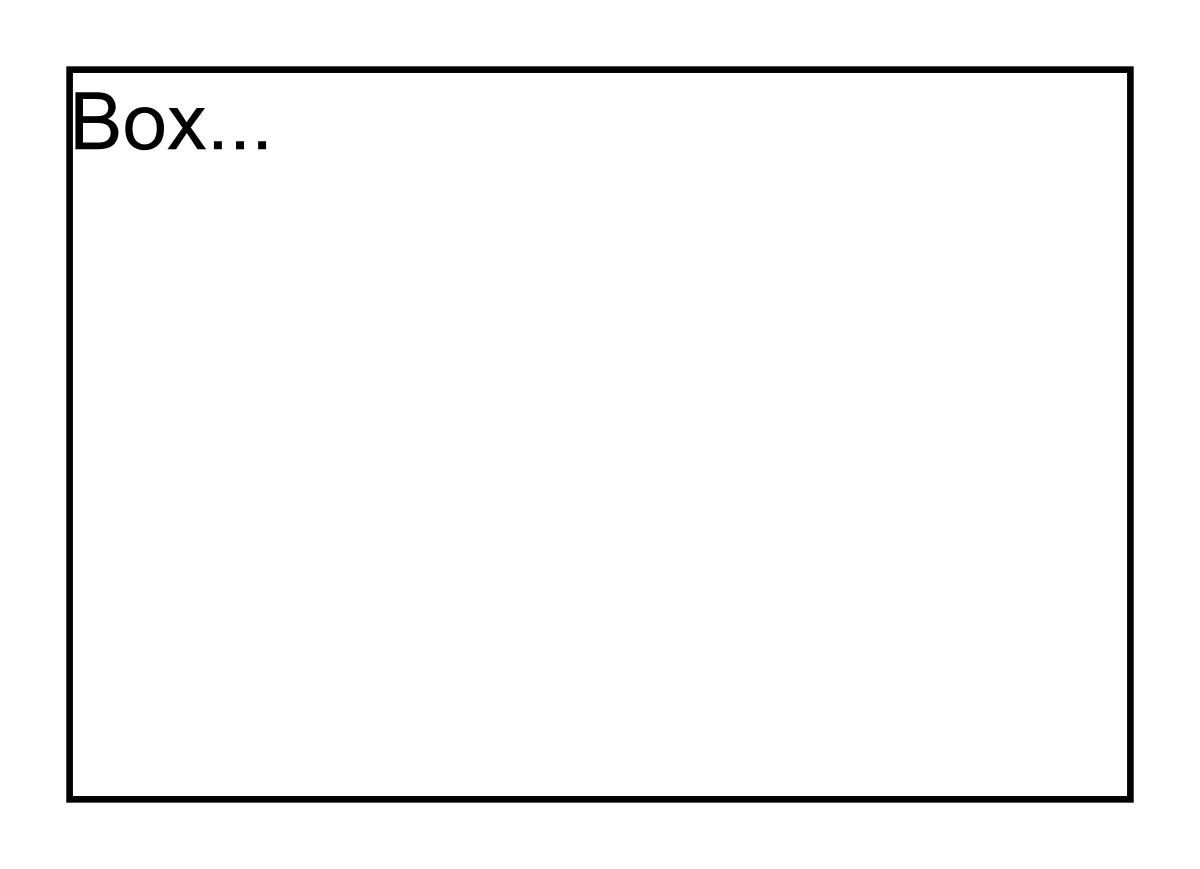
\includegraphics[width=0.5\textwidth]{Images/chapter_17/section_5732015845670912/5948595281723392.png}
 \caption{The class diagram of the Box class}
\end{figure}

\subsubsection{Chessboard}\label{kuvQVwjnsywpoEp6iam-9}
\\
The \texttt{Chessboard} models the 8x8 grid of boxes. It maintains the game's current state, including all pieces and their positions. The board is responsible for resetting and updating itself according to the moves played.

\begin{figure}[htbp]
 \centering
 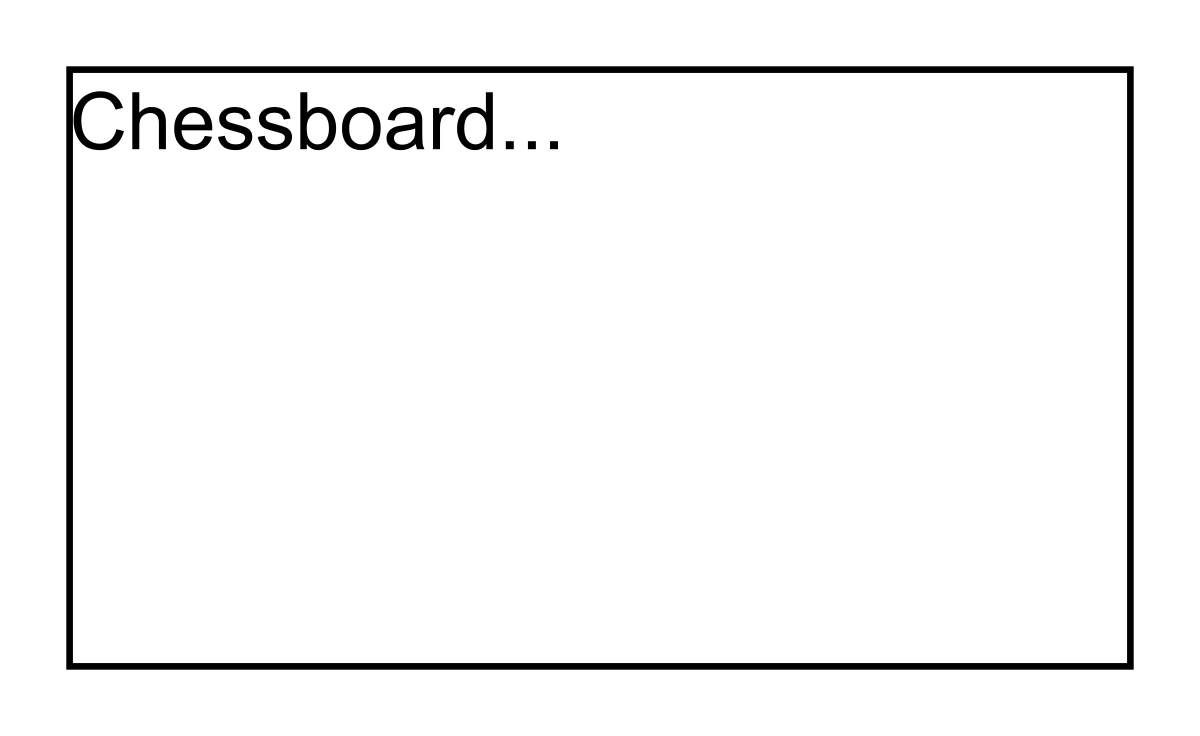
\includegraphics[width=0.5\textwidth]{Images/chapter_17/section_5732015845670912/6230399846842368.png}
 \caption{The class diagram of the Chessboard class}
\end{figure}

\subsubsection{Piece}\label{KRPjT1mRzwlc5ngJf_y9B}
\\
A \texttt{Piece} represents any chess piece (king, queen, rook, bishop, knight, or pawn) with a color (black or white) and an ``alive'' or ``captured'' status.

\begin{itemize}
\item
\protect\phantomsection\label{auyRtLg-DQ4zjZq-4xJdO}
\texttt{King}, \texttt{Queen}, \texttt{Rook}, \texttt{Bishop}, \texttt{Knight}, and \texttt{Pawn} are subclasses of \texttt{Piece}, each implementing its specific movement logic and special rules (e.g., castling for \texttt{King}/\texttt{Rook}, en passant, and promotion for \texttt{Pawn}).
\end{itemize}

\begin{figure}[htbp]
 \centering
 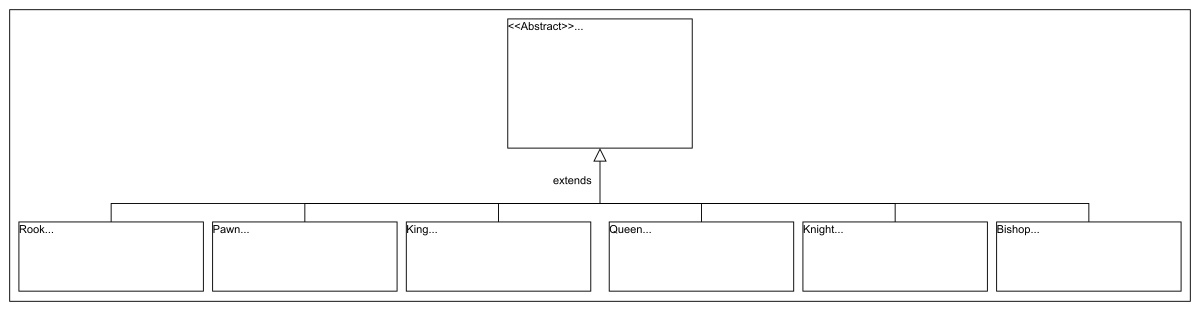
\includegraphics[width=0.5\textwidth]{Images/chapter_17/section_5732015845670912/6215747549134848.png}
 \caption{The class diagram of the Piece and its derived classes}
\end{figure}

\textbf{R4:} At the start of the game, each player will have eight pawns, two rooks, two bishops, two knights, one queen, and one king on the board.

\subsubsection{Move}\label{_VMZXbSn8D_u3kYhxXJ-B}
\\
A \texttt{Move} represents the transfer of a piece from one box to another, possibly capturing an opponent's piece. The
\texttt{Move} class tracks information such as the source and destination boxes, the moved piece, any captured piece, and whether the move resulted in special actions (e.g., castling, promotion).

\begin{figure}[htbp]
 \centering
 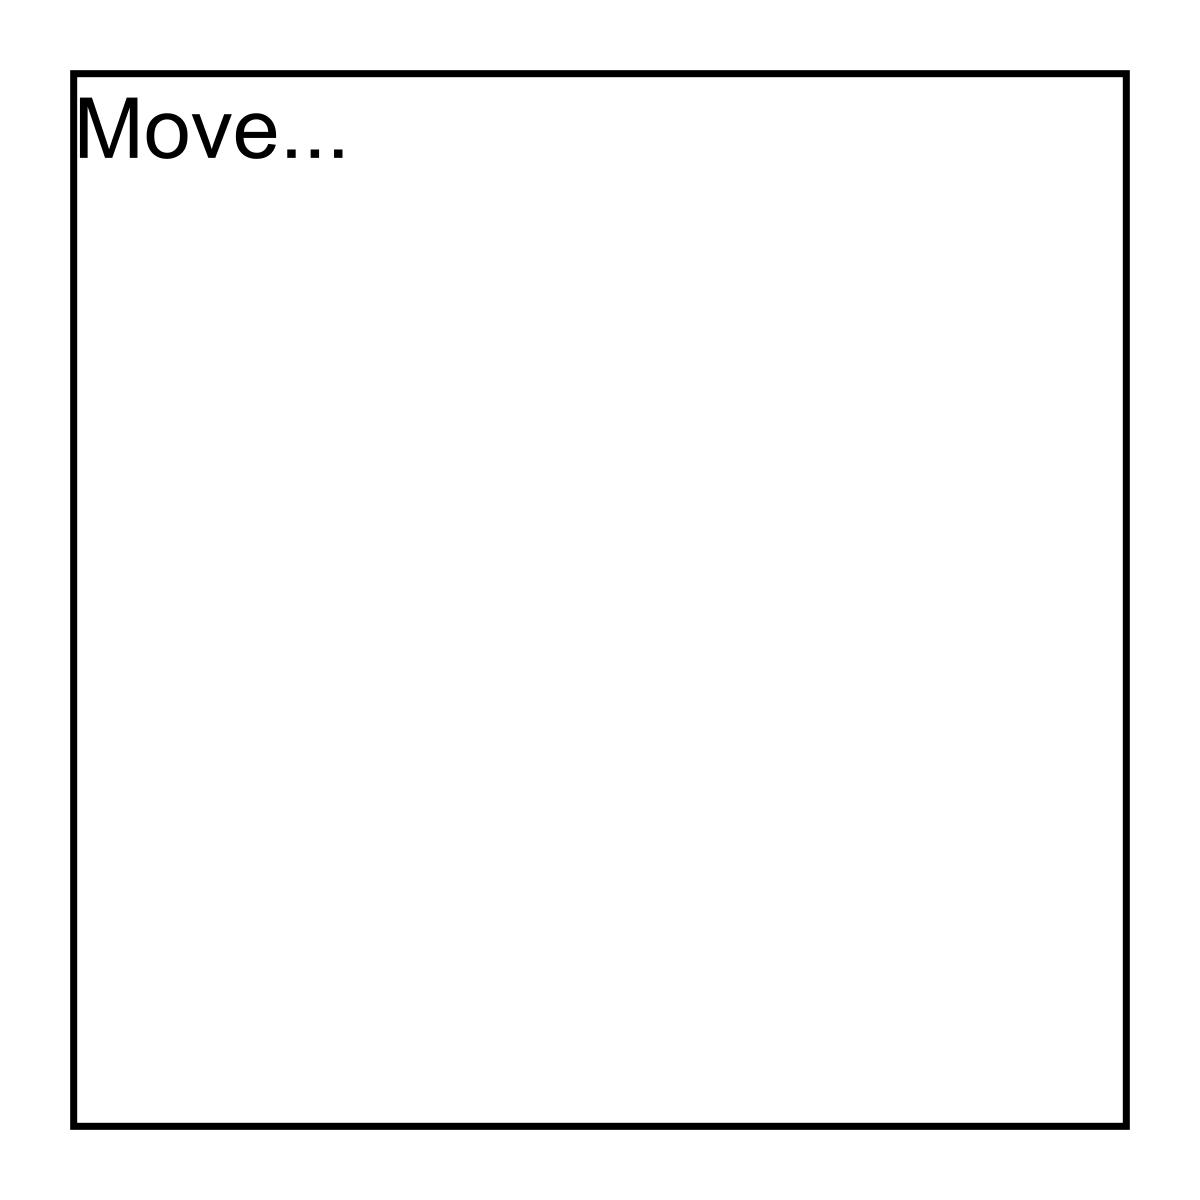
\includegraphics[width=0.5\textwidth]{Images/chapter_17/section_5732015845670912/4873044353744896.png}
 \caption{The class diagram of the Move class}
\end{figure}

\textbf{R5:} The player with the white pieces will make the first move.
\\
\textbf{R6:} Once a move has been made, a player cannot retract or undo it.

\subsubsection{Player}\label{6Q6Wzn82dpjV4b43ACSmN}
\\
The \texttt{Player} represents one of the two participants in the game, associated with a color (white or black). The
\texttt{Player} class is responsible for making moves and can resign or forfeit the game. Each player can review the game state and history.

\begin{figure}[htbp]
 \centering
 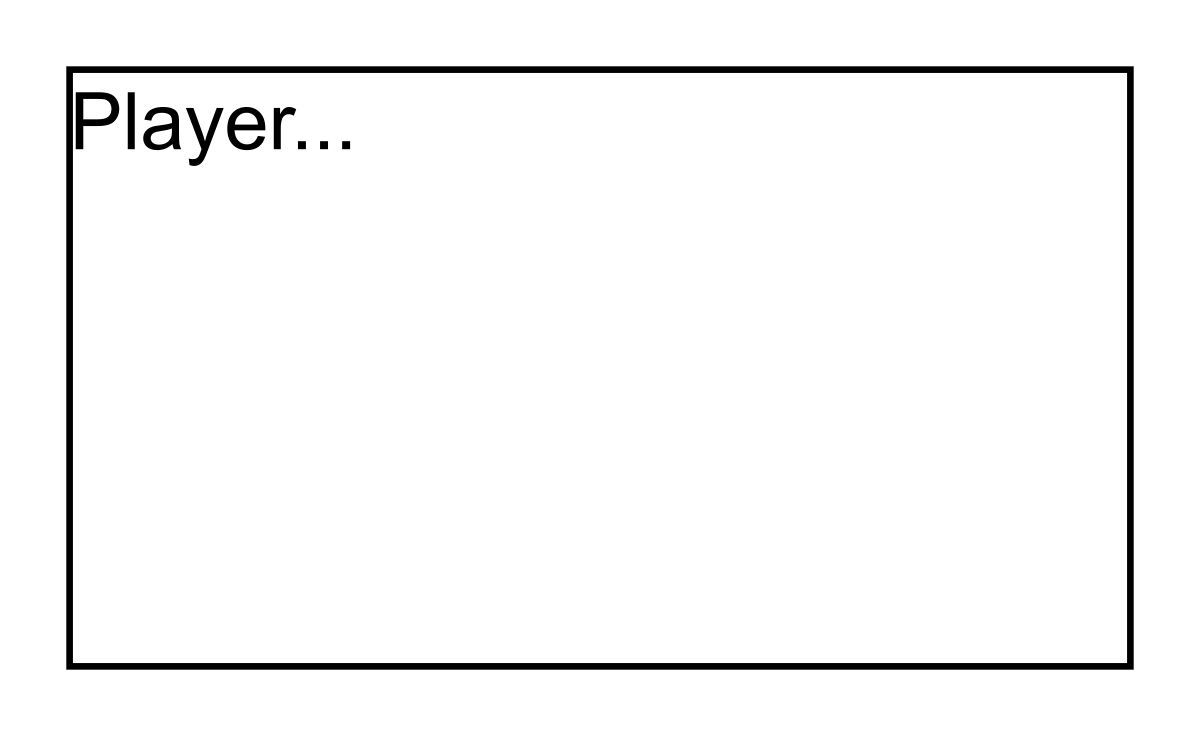
\includegraphics[width=0.5\textwidth]{Images/chapter_17/section_5732015845670912/5431469944995840.png}
 \caption{The class diagram of Player and its derived classes}
\end{figure}

\textbf{R1:} This system enables \#key\# multiplayer: A game that can be against the CPU or an online opponent. \#key\# in a game of chess via an online platform.

\subsubsection{Chess move controller}\label{r0sm9vumJHSfncy717gP0}
\\
The \texttt{ChessMoveController} encapsulates the logic for validating moves according to chess rules. It checks if a move is legal, applies it if valid, and communicates with the game to update the state. It handles rule enforcement, including check, checkmate, stalemate, castling, en passant, and promotion.

\begin{figure}[htbp]
 \centering
 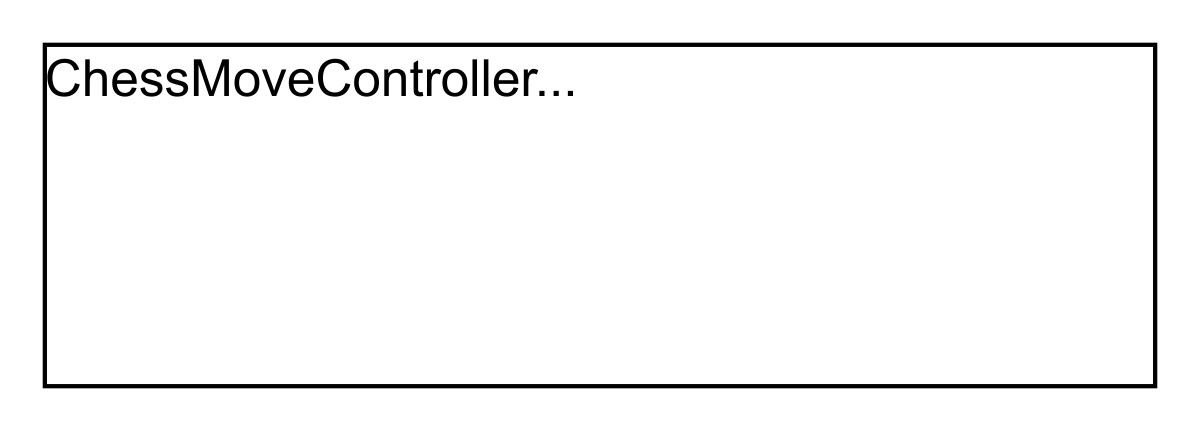
\includegraphics[width=0.5\textwidth]{Images/chapter_17/section_5732015845670912/5965961445113856.png}
 \caption{The class diagram of the ChessMoveController class}
\end{figure}

\textbf{R2:} The game will be played according to the official rules of an international chess game.

\subsubsection{Chess game view}\label{tM221oC9Fc6Cg0q5vbL0J}
\\
The \texttt{ChessGameView} is responsible for presenting the game\textquotesingle s current state---board, moves, and status---to the players (e.g., through a UI or console output).

\begin{figure}[htbp]
 \centering
 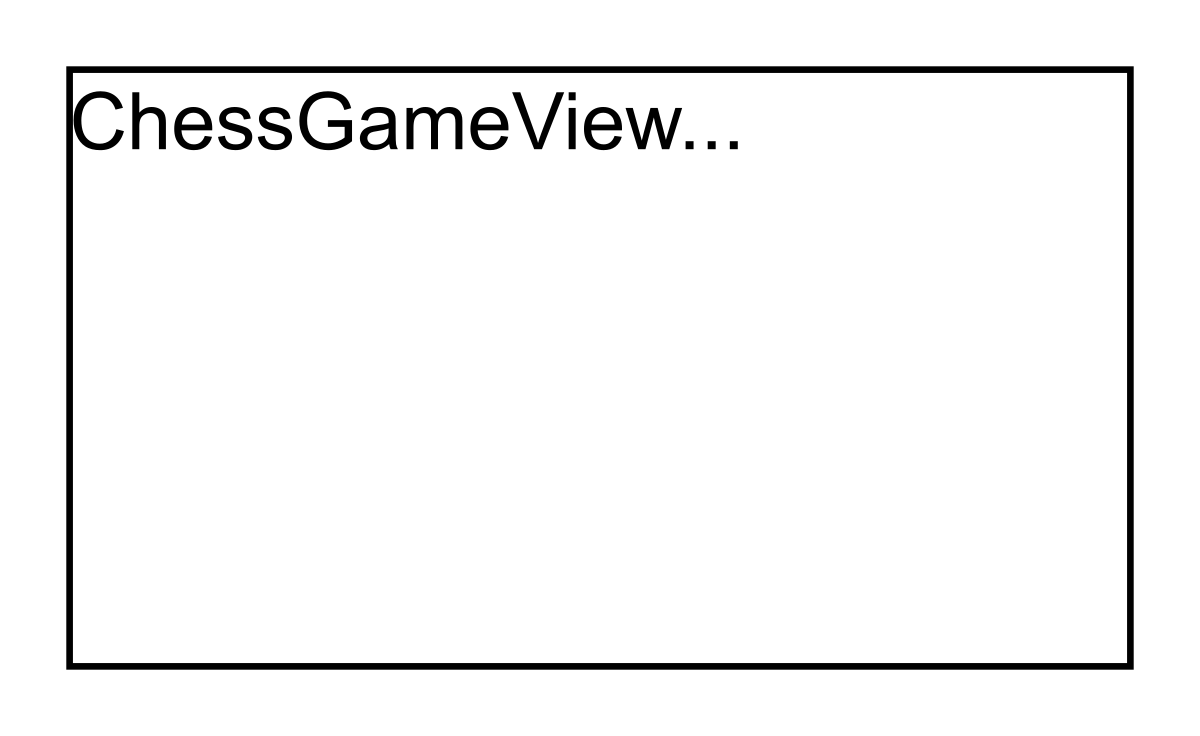
\includegraphics[width=0.5\textwidth]{Images/chapter_17/section_5732015845670912/5466236849618944.png}
 \caption{The class diagram of the ChessGameView class}
\end{figure}

\subsubsection{Chess game}\label{oc3f603stwGye80Y2LwDc}
\\
The \texttt{ChessGame} coordinates the gameplay, tracking both players, the current board, move history, and the game's status (in progress, checkmate, draw, etc.). It processes player turns, applies moves, and determines game outcomes.

\begin{figure}[htbp]
 \centering
 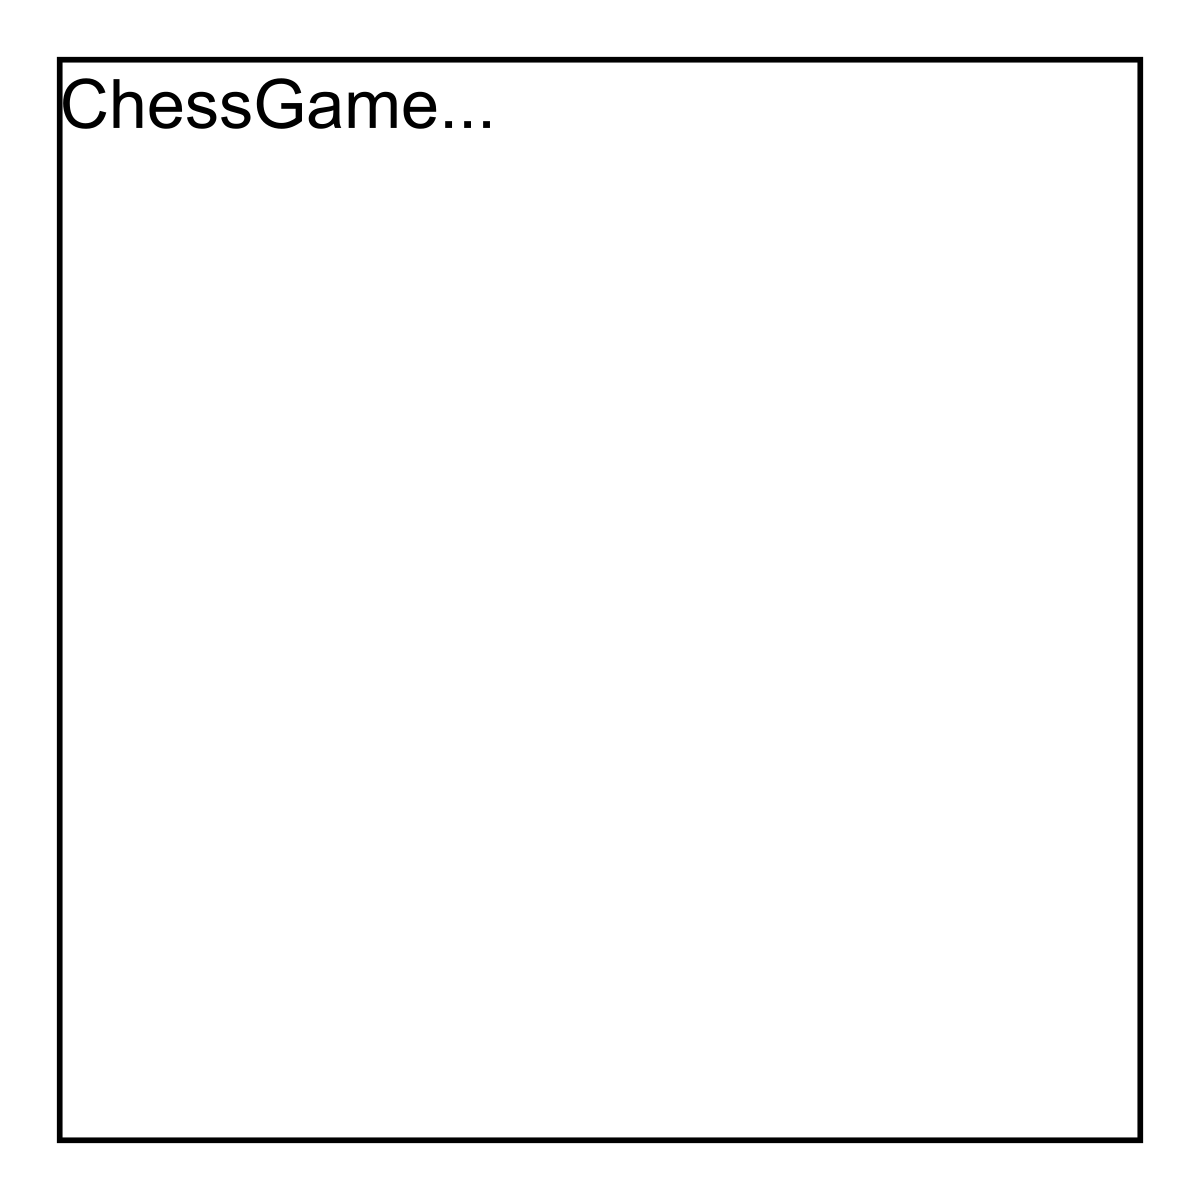
\includegraphics[width=0.5\textwidth]{Images/chapter_17/section_5732015845670912/5838056664727552.png}
 \caption{The ChessGame class}
\end{figure}

\subsubsection{Enumerations and custom data types}\label{MWdMsKN-a5RBDxDdmvW0X}
\\
The enumerations and custom data types required in the chess game design problem are listed below:

\begin{itemize}
\item
\protect\phantomsection\label{PGCvpRohGYdAJi3rKm-H_}
\textbf{GameStatus:} Tracks the current game state (in progress, white wins, black wins, draw, etc.).
\item
\protect\phantomsection\label{wqW3iSTgPrm6-UhDxhkzv}
\textbf{MoveType:} Enum for regular, castling, en passant, promotion, etc.
\end{itemize}

\begin{figure}[htbp]
 \centering
 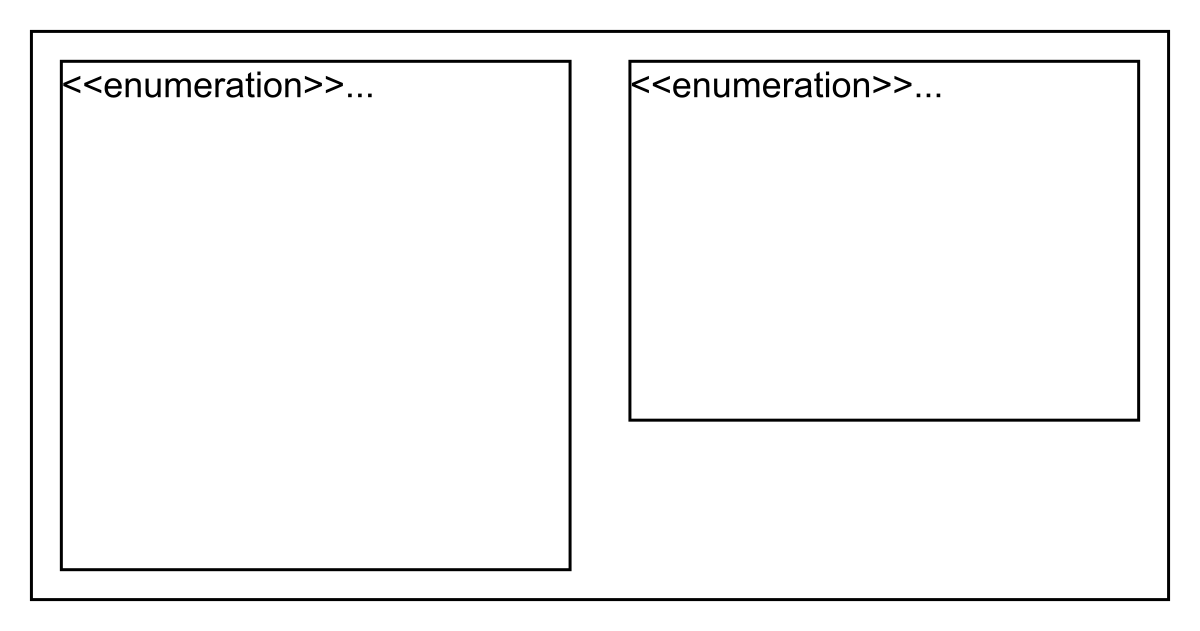
\includegraphics[width=0.5\textwidth]{Images/chapter_17/section_5732015845670912/4679476217511936.png}
 \caption{The class diagram of the Person class}
\end{figure}

\subsection{Relationship between the classes}\label{lTqA4q4Rq1gELYLeamRjz-3}
\\
Now, we'll discuss the relationships between the classes we have defined above for our chess game design.

\subsubsection{Association}\label{obyktukAe7kxWeXZ56AO3}
\\
The class diagram has the following association relationships:

\begin{itemize}
\item
\protect\phantomsection\label{YIOxcjDb69GElBYVH-BC-}
The \texttt{Move} class has a one-way association with \texttt{Player}, \texttt{Piece}, and \texttt{Box} (each move is linked to the player making the move, the piece moved, the captured piece (if any), and the start/end boxes).
\item
\protect\phantomsection\label{kAwUrxD0YniFLJK8JkkfC}
The \texttt{ChessGame} class has a one-way association with \texttt{ChessMoveController} (for move validation).
\item
\protect\phantomsection\label{bCa_m-h4A9uixgf1qOEK8}
The \texttt{ChessGame} class has a one-way association with \texttt{ChessGameView} (for updating the view/display).
\item
\protect\phantomsection\label{jNZLOC-YsImViZCofefyH}
The \texttt{ChessMoveController} class has a one-way association with \texttt{ChessGame} (to access the game state/board as needed).
\item
\protect\phantomsection\label{lh_fLzGgEgUO4iUDLFyNA}
The \texttt{ChessGameView} class has a one-way association with \texttt{ChessGame} or \texttt{Chessboard} (to display the current game state).
\end{itemize}

\begin{figure}[htbp]
 \centering
 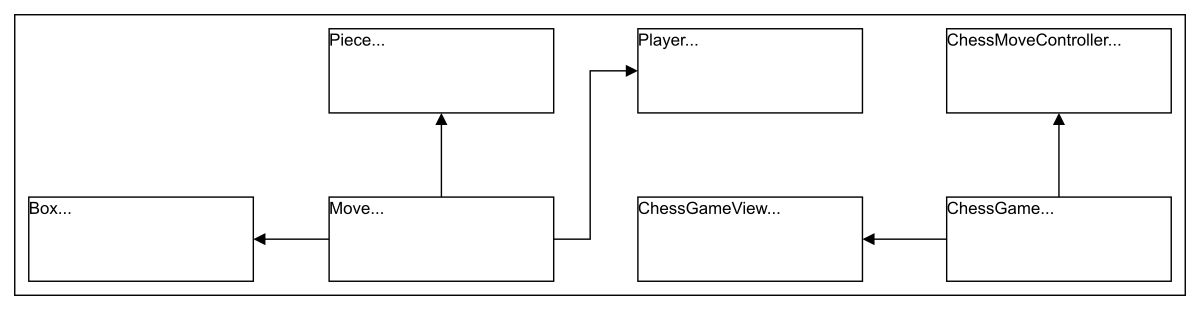
\includegraphics[width=0.5\textwidth]{Images/chapter_17/section_5732015845670912/5845759973785600.png}
 \caption{The association relationship between classes}
\end{figure}

\subsubsection{Aggregation}\label{noyU8seJ0WVmxVLWh59zu}
\\
The class diagram has the following aggregation relationships:

\begin{itemize}
\item
\protect\phantomsection\label{pzC0vmBk3dFO0TL3j2Mx2}
The \texttt{ChessGame} class aggregates two \texttt{Player} objects (white and black).

\begin{itemize}
\item
(Players are part of a game but exist independently and can participate in other games.)
\end{itemize}
\end{itemize}

\begin{figure}[htbp]
 \centering
 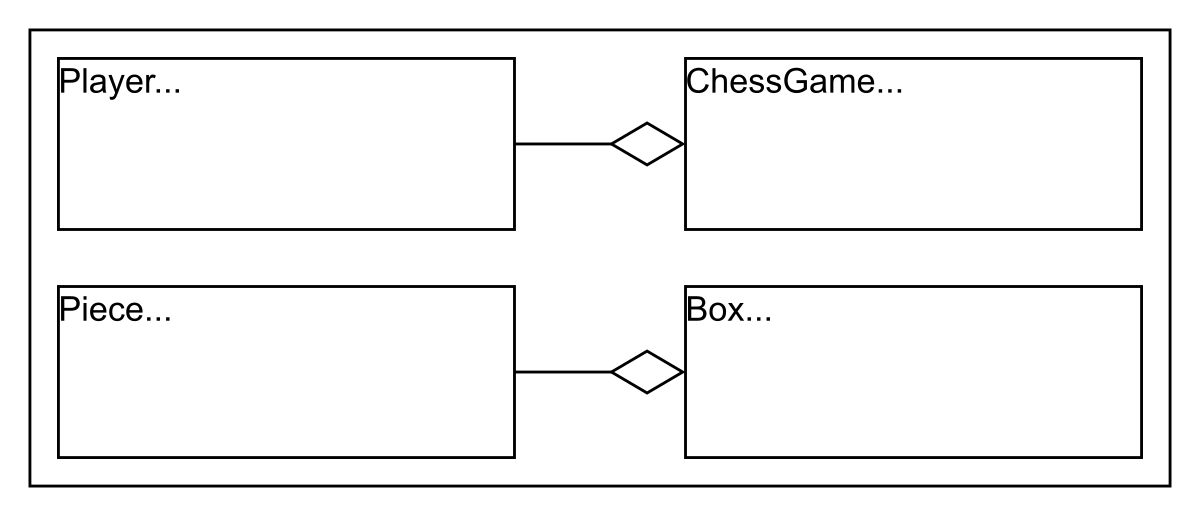
\includegraphics[width=0.5\textwidth]{Images/chapter_17/section_5732015845670912/6290480802168832.png}
 \caption{The aggregation relationship between classes}
\end{figure}

\subsubsection{Composition}\label{j9LKUkNT_QebF_q9mWfLi}
\\
The class diagram has the following composition relationships.

\begin{itemize}
\item
\protect\phantomsection\label{VmAuFr7cq_UWoFaQAu89E}
The \texttt{ChessGame} class is composed of a \texttt{Chessboard} and a collection of \texttt{Move} objects (the game controls their lifecycle).
\item
\protect\phantomsection\label{Dn6OTYj-8-mCvT82Lz12X}
The \texttt{Chessboard} class is composed of 64 \texttt{Box} objects (boxes only exist as part of a board).
\item
\protect\phantomsection\label{jHM4UwXsAZniRozXJ2SS0}
Each \texttt{Box} may be composed of a \texttt{Piece} (a piece lives in a box; if removed from the board, it's no longer in play).
\end{itemize}

\begin{figure}[htbp]
 \centering
 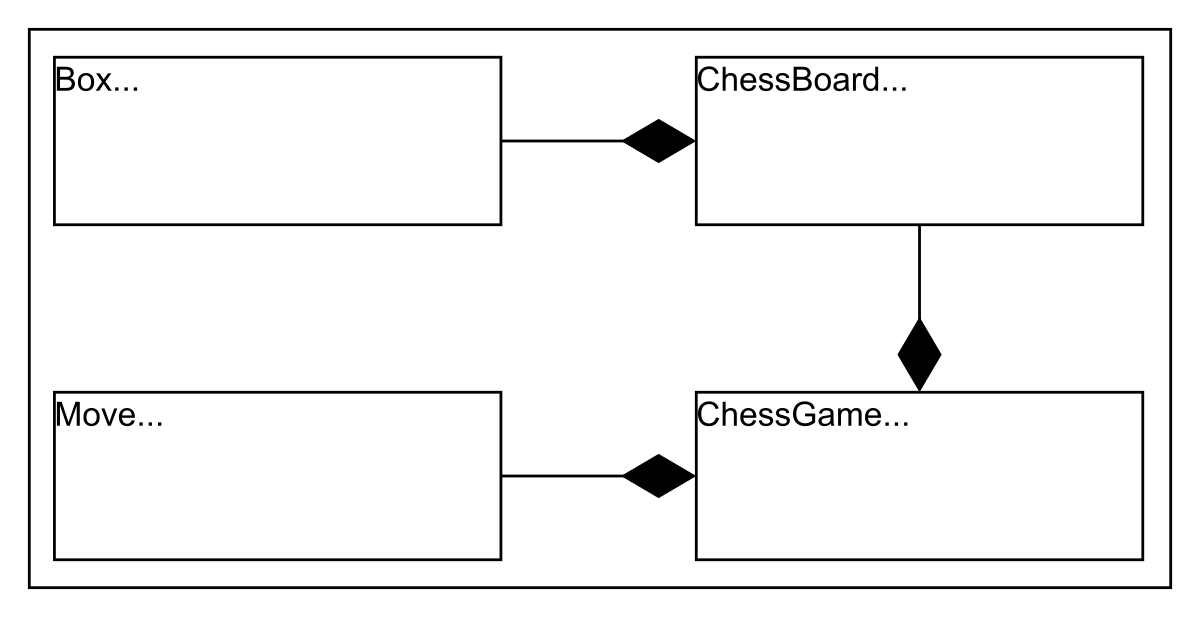
\includegraphics[width=0.5\textwidth]{Images/chapter_17/section_5732015845670912/5930694613008384.png}
 \caption{The composition relationship between classes}
\end{figure}

\subsubsection{Inheritance}\label{VB-a0gzbl1Vlz8sozqCrS}
\\
The following classes demonstrate an inheritance relationship:

\begin{itemize}
\item
\protect\phantomsection\label{lHzZjDU9TWWeeRvDEhsEJ}
The \texttt{King}, \texttt{Queen}, \texttt{Rook}, \texttt{Bishop}, \texttt{Knight}, and \texttt{Pawn} classes extend the \texttt{Piece} class.
\end{itemize}
\begin{quote}
\textbf{Note:} We have already discussed the inheritance relationship between classes in the component section above one by one.
\end{quote}
\subsection{Class diagram for the chess game}\label{_J1DMnFsFt0FoyHnpKEiO}
\\
This section outlines the multiplicity (cardinality) relationships between the main classes in our chess game. We explain the allowed number of instances on each side for each relationship and the real-world or design rationale behind the connection. Understanding these relationships is key to modeling how different entities interact and collaborate to support key workflows in the system.

\begin{table}[h!]
\centering
\begin{tabular}{|p{3.5cm}|p{3.5cm}|p{3cm}|p{6.5cm}|}
\hline
\textbf{Source} & \textbf{Target} & \textbf{Multiplicity} & \textbf{Reason} \\
\hline
ChessGame & ChessBoard & 1--1 & Each game has exactly one chessboard. \\
\hline
ChessGame & Player & 1--2 & Each game has two players (white and black). \\
\hline
ChessGame & Move & 1--0..* & Each game can have zero or more moves (move history). \\
\hline
ChessGame & ChessMoveController & 1--1 & Each game uses one move controller. \\
\hline
ChessGame & ChessGameView & 1--1 & Each game uses one view to display the game state. \\
\hline
ChessBoard & Box & 1--64 & Each board consists of exactly 64 boxes (8$\times$8 grid). \\
\hline
Box & Piece & 0..1--0..1 & Each box may contain at most one piece, and a piece is in at most one box at a time. \\
\hline
Move & Player & 1--1 & Each move is made by exactly one player. \\
\hline
Move & Box & 1--2 & Each move is associated with a start box and an end box. \\
\hline
Move & Piece & 1..2--1 & Each move references one piece moved and possibly one piece captured. \\
\hline
\end{tabular}
\caption{Entity Relationships and Multiplicities in a Chess Game}
\label{tab:chess_entity_relationships}
\end{table}


Here's the complete class diagram for our chess game:

\begin{figure}[htbp]
 \centering
 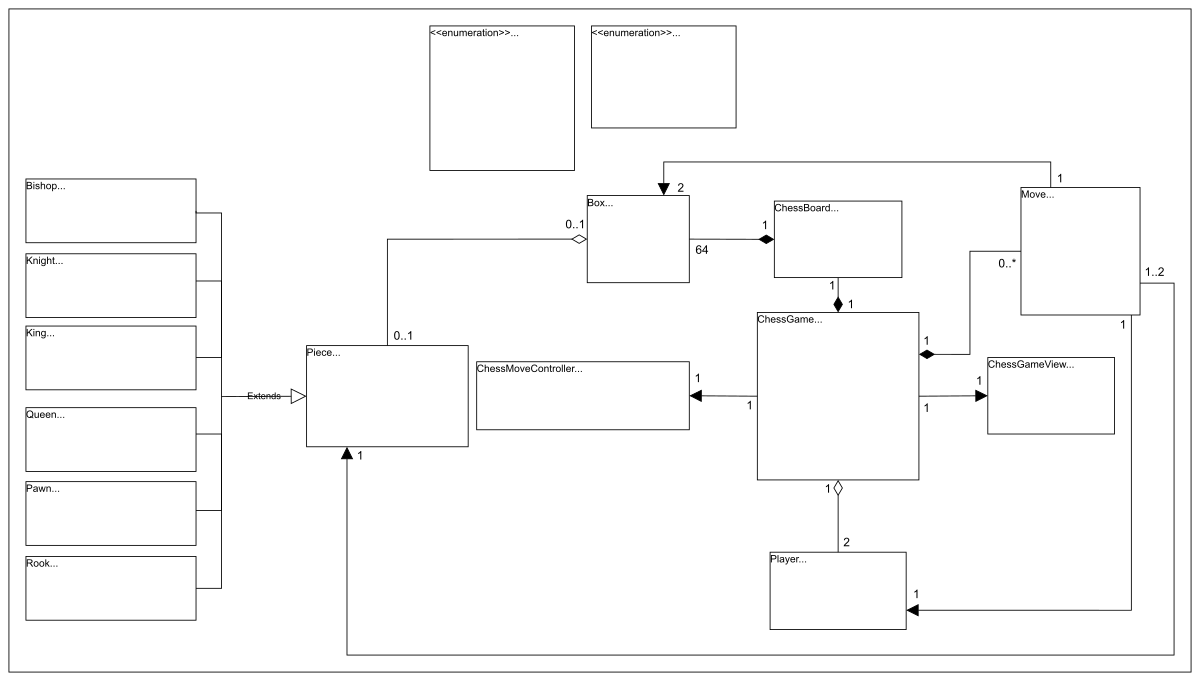
\includegraphics[width=0.5\textwidth]{Images/chapter_17/section_5732015845670912/4763164288614400.png}
 \caption{The class diagram of the chess game}
\end{figure}

\subsection{Design pattern}\label{1JdnBslPYoJ3idant5lQ4}
\\
The following design patterns have been used in the class diagram:

\begin{itemize}
\item
\protect\phantomsection\label{Fms8jhb8iluIuZwvrdivT}
\textbf{Singleton design pattern:} This pattern ensures the existence of a single instance of the chessboard at a given moment due to the shared nature of the chessboard as a resource. Multiple instances can cause the game state to become inconsistent.
\item
\protect\phantomsection\label{NTfR4jqKyjZGL7a4LzvfF}
\textbf{Command design pattern:} This pattern encapsulates the move logic for each chess piece. Each piece has its own implementation of the move command, which allows it to move according to the rules defined for it. For example, the knight moves in an L-shape pattern, or the rook can move only horizontally or vertically on any number of boxes.
\end{itemize}
\\
The following design patterns can also be used to design chess:

\begin{itemize}
\item
\protect\phantomsection\label{fvhLyuhnlQJvv-vwT0eXN}
The Iterator design pattern would enable the game to move sequentially by allowing the pieces to behave uniformly, where the user does not need to know the specifications or underlying logic behind the moves of the pieces.
\item
\protect\phantomsection\label{OA03GuyCRYxEg8LZbfkGE}
The State design pattern ensures the encapsulation of each piece's state logic since all the chess pieces have their own respective implementations of checkmate states, which cause them to behave differently depending on the situation.
\item
\protect\phantomsection\label{53q4JA-ByaW0JHY_26hqh}
The Observer design pattern enables the chess pieces to act as observers when the chessboard is the subject. As soon as the board's state changes, the pieces are notified to adapt accordingly, decoupling them from the board.
\end{itemize}

\subsection{AI-powered trainer}\label{YNYvDRpgBMvmSK5eg1cwQ}
\\
At this stage, everything should be clear. If you encounter any confusion or ambiguity, feel free to utilize the interactive AI-enabled widget below to seek clarification. This tool is designed to help you strengthen your understanding of the concepts.

\begin{figure}[htbp]
 \centering
 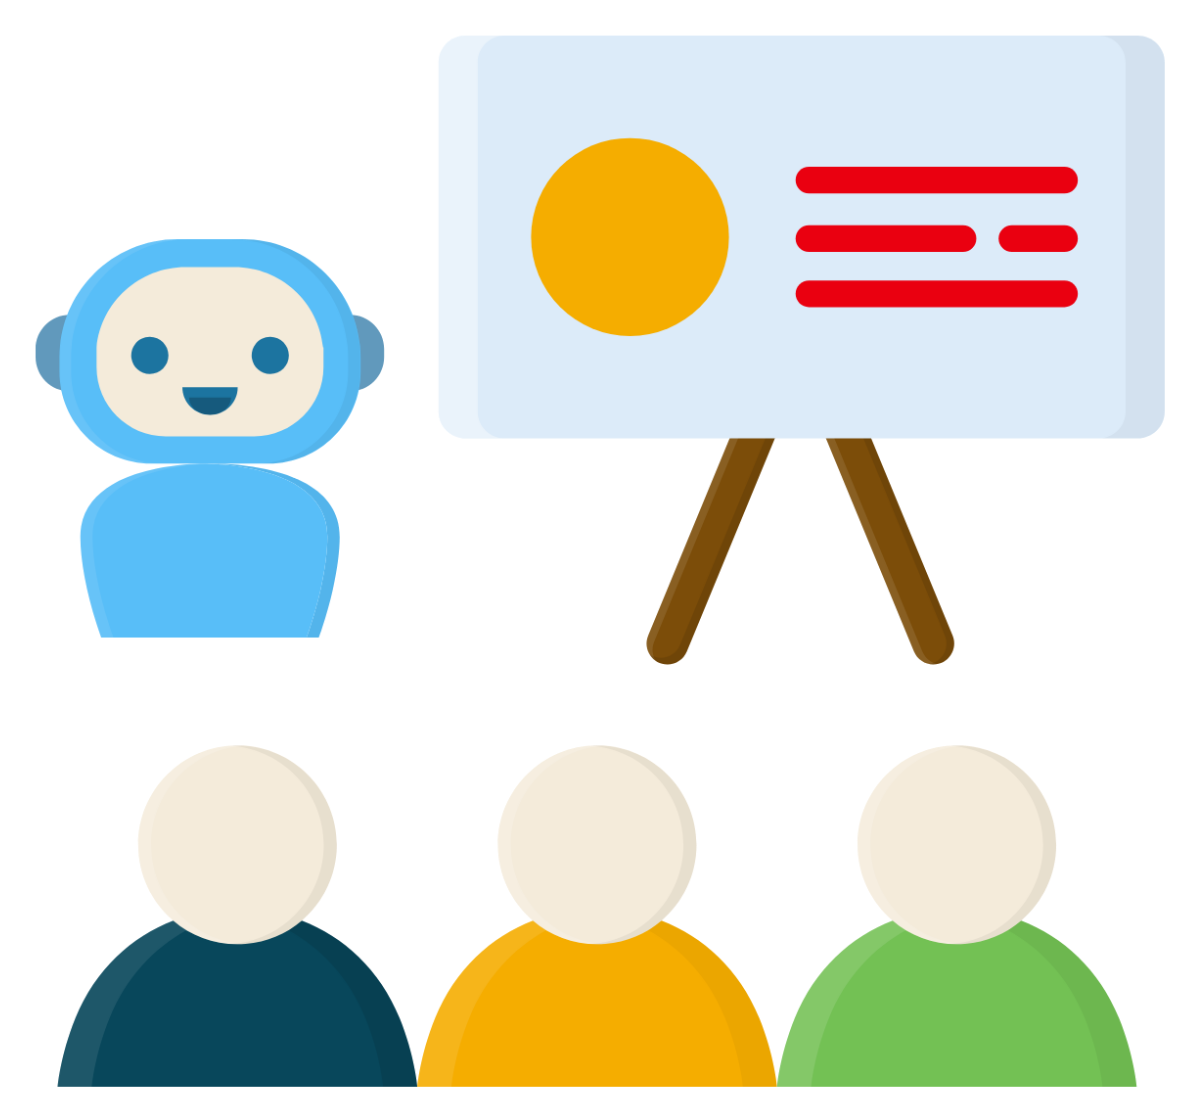
\includegraphics[width=0.15\textwidth]{Images/chapter_17/section_5732015845670912/5112358517997568.png}
 
\end{figure}

We have completed the class diagram of the chess game according to the requirements. In the next lesson, let's design its activity diagram.

% End of section content